\begin{mydefs}
	\begin{itemize}
		\item Si les cotés de l'angle sont confondus, l'angle est \kw{nul}.
		
		
		\item Si l'angle est plus petit qu'un angle droit, l'angle est \kw{aigu}.
		
		\item Si les cotés sont perpendiculaires, l'angle est \kw{droit}.
		
		\item Si l'angle est plus grand qu'un angle droit, l'angle est \kw{obtus}.		
		
		\item Si les cotés sont dans le prolongement l'un de l'autre, l'angle est \kw{plat}.
	\end{itemize}
\end{mydefs}

\begin{myexs}
	\begin{itemize}
		
			

	
		\item L'angle $\widehat{ABC}$ est nul.
			\begin{center}
				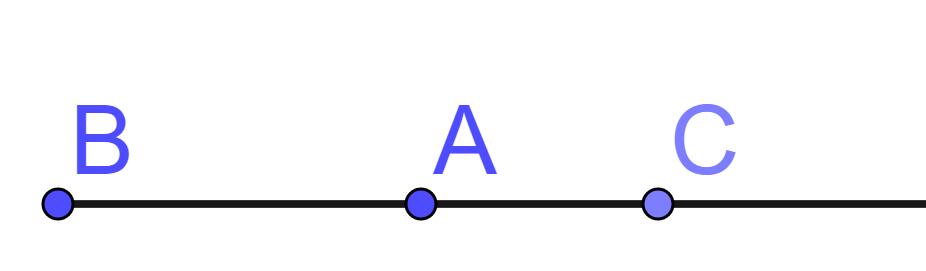
\includegraphics[scale=0.2]{angle_nul}
			\end{center}
		
		\begin{multicols}{2}
		\item L'angle $\widehat{DEF}$ est aigu.
			\begin{center}
				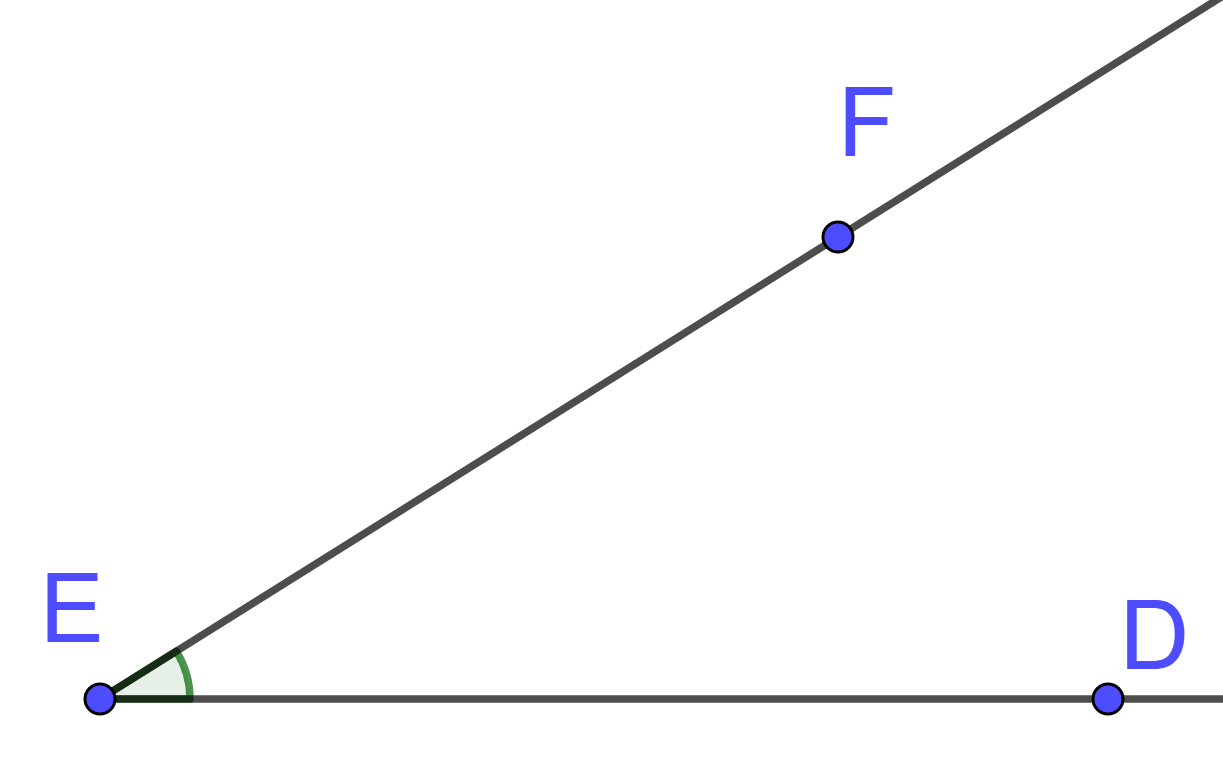
\includegraphics[scale=0.2]{aigu}
			\end{center}
		
		\item L'angle $\widehat{GHI}$ est droit.
			\begin{center}
				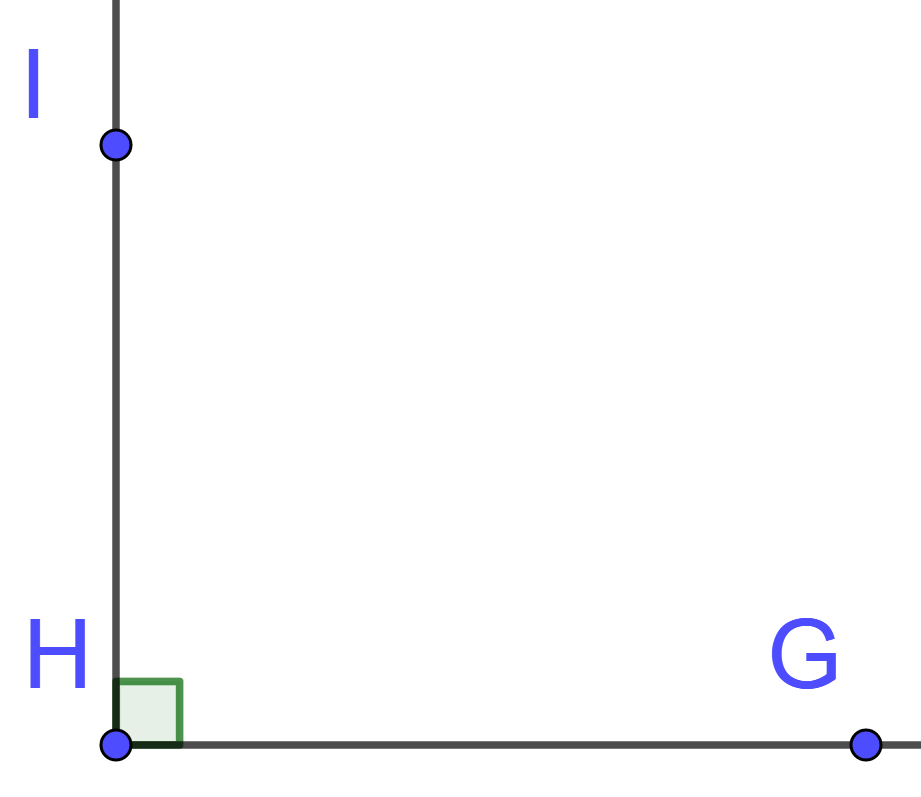
\includegraphics[scale=0.2]{droit}
			\end{center}
		
		\item L'angle $\widehat{JKL}$ est obtus.
			\begin{center}
				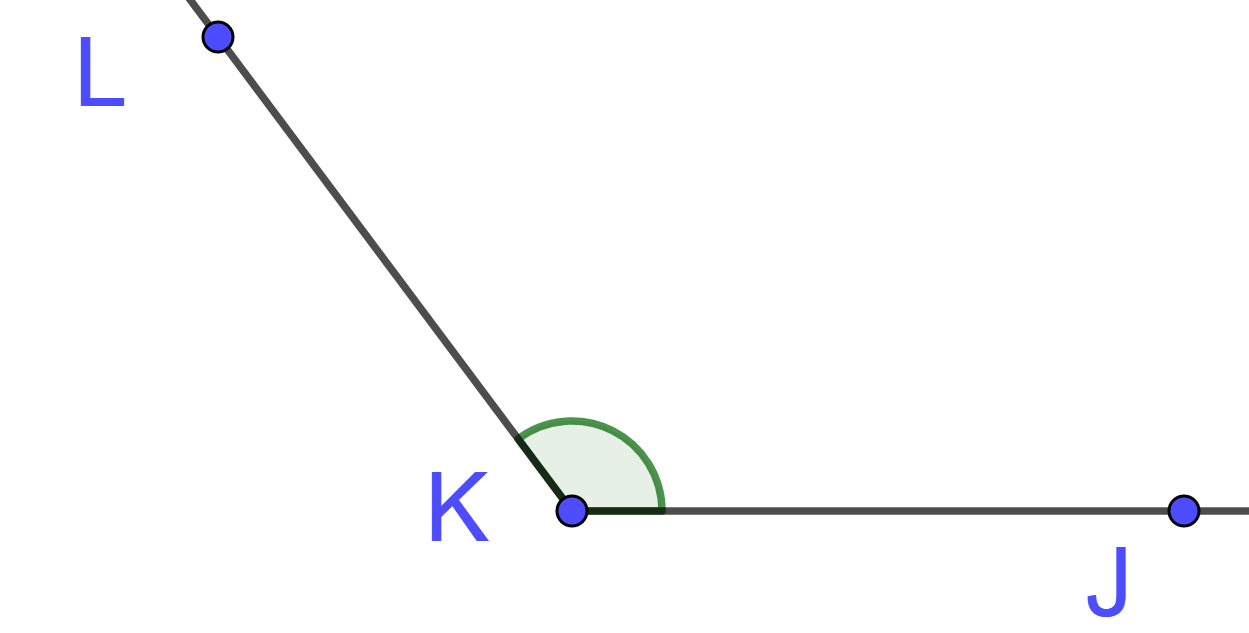
\includegraphics[scale=0.2]{obtus}
			\end{center}
		
		\item L'angle $\widehat{MNO}$ est plat.
			\begin{center}
				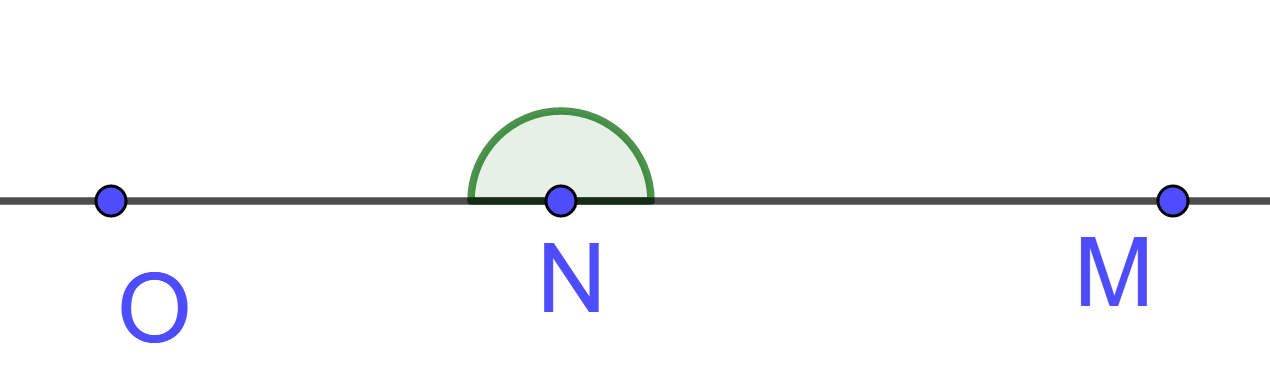
\includegraphics[scale=0.2]{plat}
			\end{center}
		\end{multicols}
	\end{itemize}
\end{myexs}